%%%%%%%%%%%%
%
% $Autor: Wings $
% $Datum: 2019-03-05 08:03:15Z $
% $Pfad: Maintenance.tex $
% $Version: 4250 $
% !TeX spellcheck = en_GB/de_DE
% !TeX encoding = utf8
% !TeX root = manual 
% !TeX TXS-program:bibliography = txs:///biber
%
%%%%%%%%%%%%

\chapter{Introduction}

Welcome to the Face Recognition for Access Control System Manual. This system uses the Arduino Portenta H7 and Vision Shield, along with Edge Impulse Studio, to deliver an efficient and accurate face recognition solution for access control. Our system designed to ensure security and reliability using MobileNet V2 algorithms and it is ideal for applications in offices, restricted zones and other areas requiring controlled access.


This manual provides a step-by-step guide to understanding, setting up and using the face recognition system. Whether you are setting up for personal use or professional applications, this manual will help you utilize the system's functionalities efficiently.

\subsection{Key Features}

\begin{itemize}
\item \textbf{Portable and Energy-Efficient:}  
Powered by the Arduino Portenta H7, the system is compact, energy-efficient and easy to set up, making it perfect for a variety of applications.
\item \textbf{Customizable User Profiles:}  
Add or remove face profiles effortlessly to keep the access control system up-to-date with changing needs.
\item \textbf{Easy Deployment:}  
Deploy trained models seamlessly on the Portenta H7, ensuring quick and hassle-free integration with the hardware.
\item \textbf{Scalable for Any Setup:}  
Whether it’s a small office or a large facility, the system can easily scale to handle varying requirements. Updating datasets and retraining models is simple and efficient.
\item \textbf{Clear and Insightful Visualizations:}  
Get a better understanding of data and model performance through detailed, easy-to-interpret visualizations.
\end{itemize}

\subsection{How to Use This Manual}

This manual is structured to provide a comprehensive guide to using the Face Recognition for Access Control System. Below is an overview of the key sections and how they can assist you:

\begin{itemize}
	\item \textbf{Introduction:}  
	Learn about the system’s purpose, key features and overall workflow.
	
	\item \textbf{Main Functionality:}  
	Get a clear understanding of how the system processes data, trains models and recognizes faces in real time.
	
	\item \textbf{Installation and Configuration:}  
	Follow detailed instructions to set up the hardware and software, install necessary tools and configure the system for use.
	
	\item \textbf{Getting Started:}  
	Learn how to prepare datasets, connect the hardware, power the system, and run the pre-installed model.
	
	\item \textbf{Maintenance:}  
	Follow guidelines to maintain hardware and update software for optimal performance.
	
	\item \textbf{Safety Guidelines:}  
	Steps to ensure safe operation with precautions for hardware, environment and data security.
	\item \textbf{Troubleshooting:} 
	Get tips to resolve some common hardware and software issues with clear solutions.
\end{itemize}


\subsection{Basic Info on the System}

The system uses the MobileNet V2 algorithm, a convolutional neural network optimized for embedded vision applications. MobileNet V2 is known for its ability to deliver high accuracy with reduced model size, making it ideal for deployment on resource-constrained devices like the Portenta H7 hardware. The CAD model of the system is listed as shown in the figure ~\ref{CAD_Model}. ALso, the GUI of the system will be available as shown in the figure ~\ref{GUI}.
\\

We are confident that our system will provide you with the tools and insights needed to effectively monitor and provide access control. If you have any questions or need further assistance, our support team is always ready to help. Let’s take a step towards smarter and more secure access control with our Face Recognition System, ensuring a seamless blend of technology and security for your environment!

\begin{figure}
	\begin{center}
		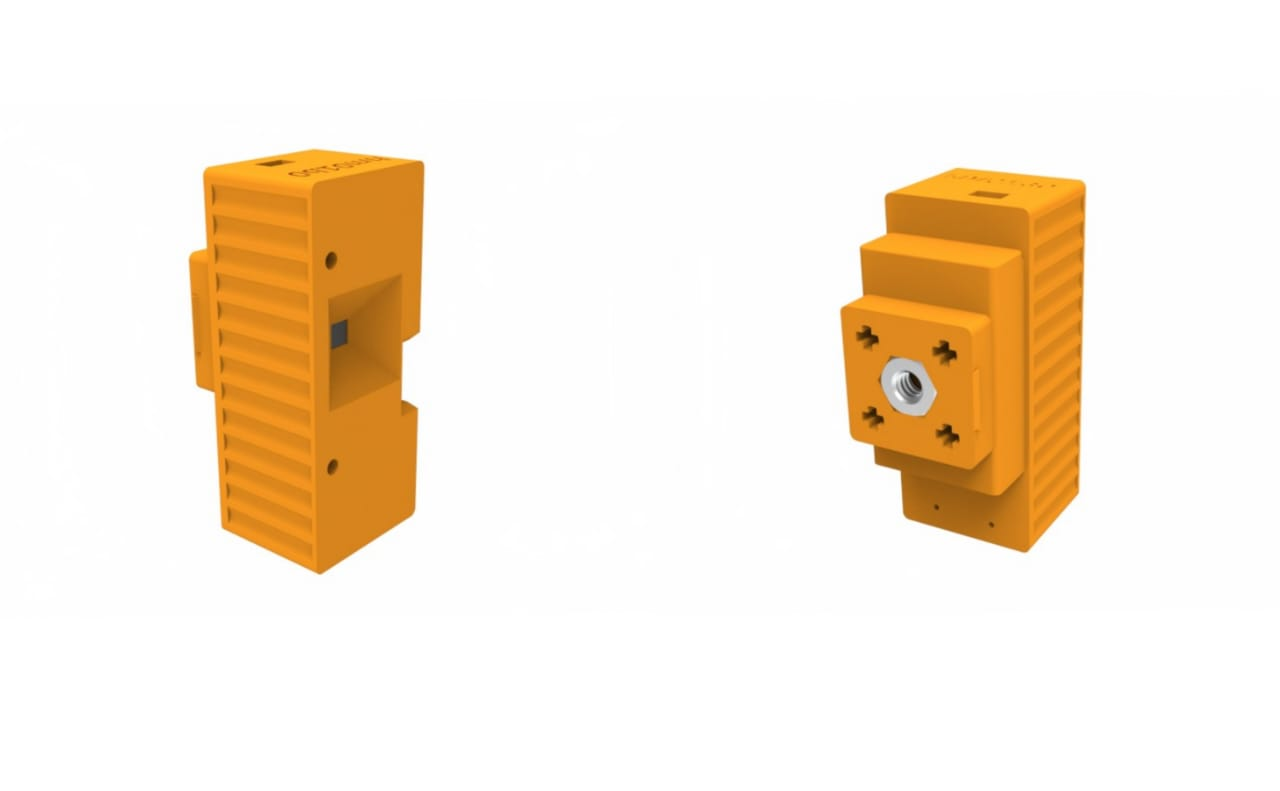
\includegraphics[width=0.7\linewidth]{Images/CAD_Model.jpg}
		\caption{CAD Model of the system}
		\label{CAD_Model}
	\end{center}
\end{figure}

\begin{figure}
	\begin{center}
		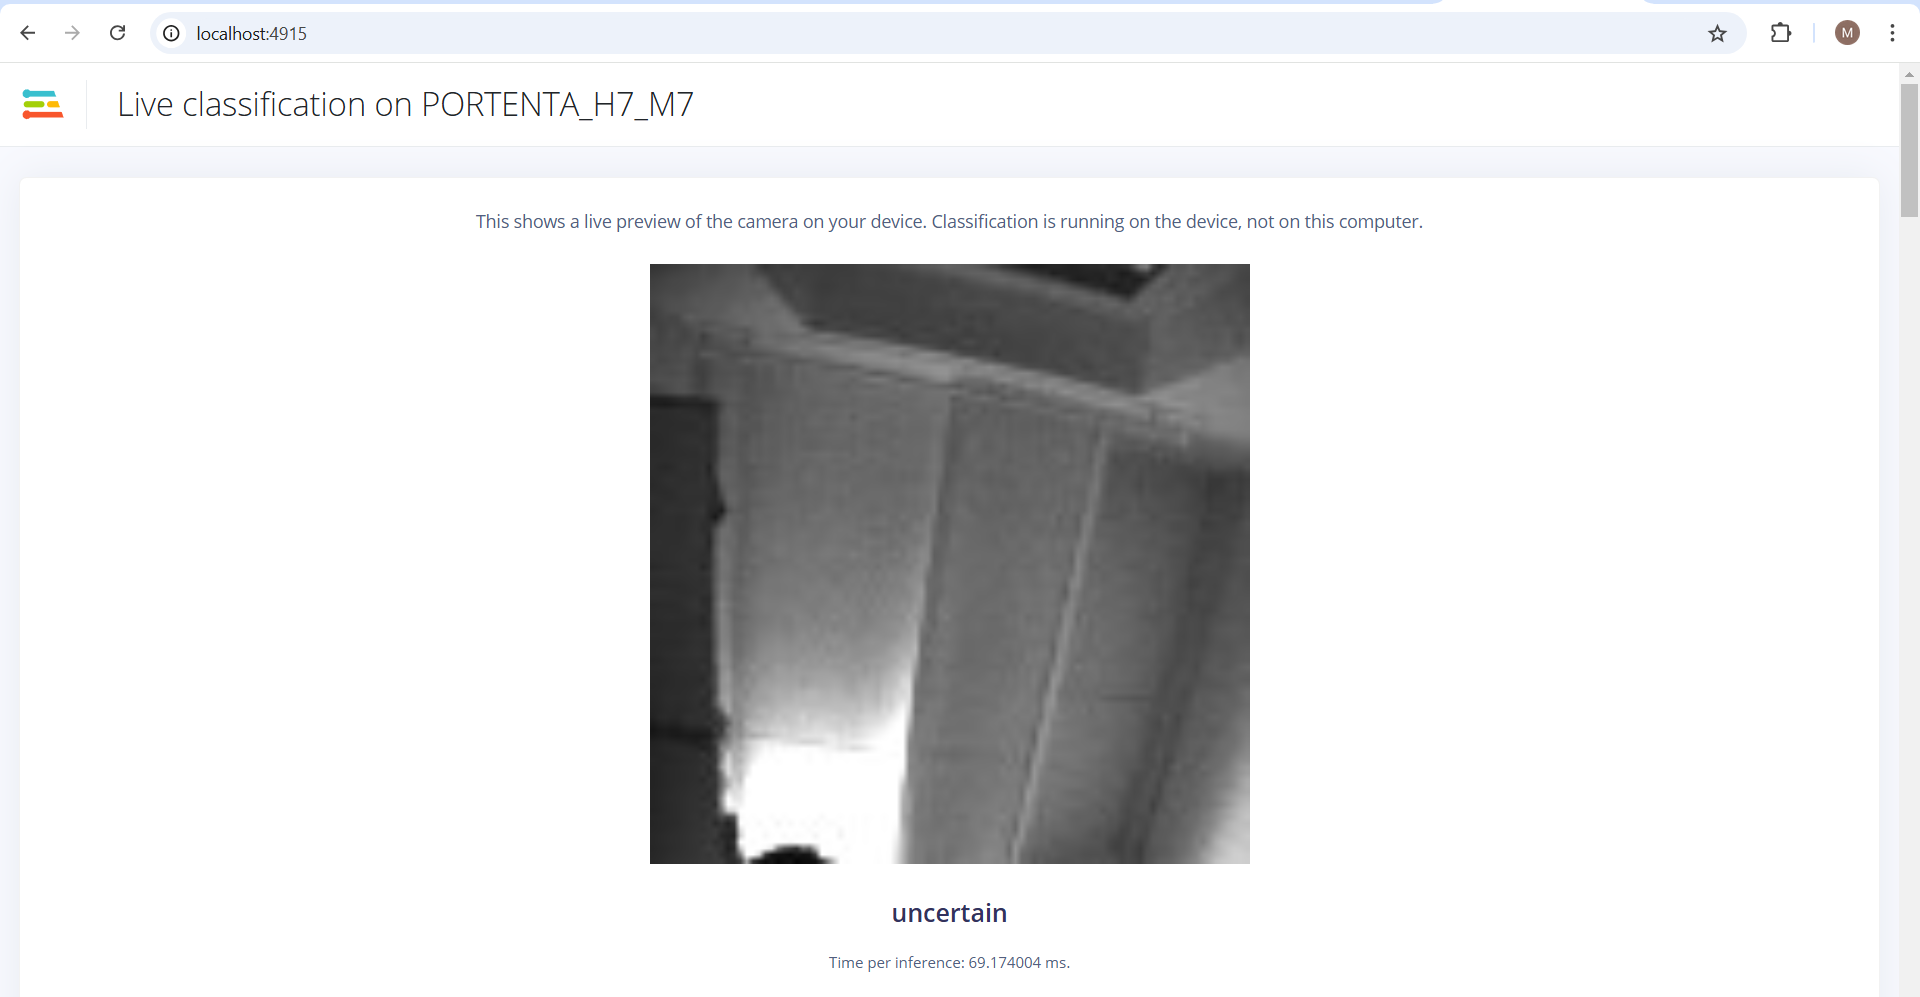
\includegraphics[width=0.7\linewidth]{Images/intro.png}
		\caption{GUI of the application}
		\label{GUI}
	\end{center}
\end{figure}